% Source: Code/xband-radar-sim/docs/radar_simulation_technical.tex
% Description: FFT-based matched filter implementation. Correlation in time domain equals multiplication in frequency domain.

\documentclass[border=4pt]{standalone}
\usepackage{algpseudocode}
\usepackage{amsmath,amssymb,amsfonts}
\usepackage[T1]{fontenc}
\usepackage{graphicx}
\usepackage{pgfplots}
\usepackage{tikz}
\usepackage{xcolor}
\pgfplotsset{compat=1.18}
\usetikzlibrary{arrows.meta,positioning,shapes.geometric,calc,patterns,decorations.pathmorphing,3d,angles,quotes}

\definecolor{radargreen}{RGB}{0,255,0}
\definecolor{raycolor}{RGB}{255,165,0}
\definecolor{targetcolor}{RGB}{255,0,0}
\definecolor{groundcolor}{RGB}{139,90,43}
\definecolor{skycolor}{RGB}{135,206,235}
\definecolor{beamcolor}{RGB}{255,255,0}


\begin{document}
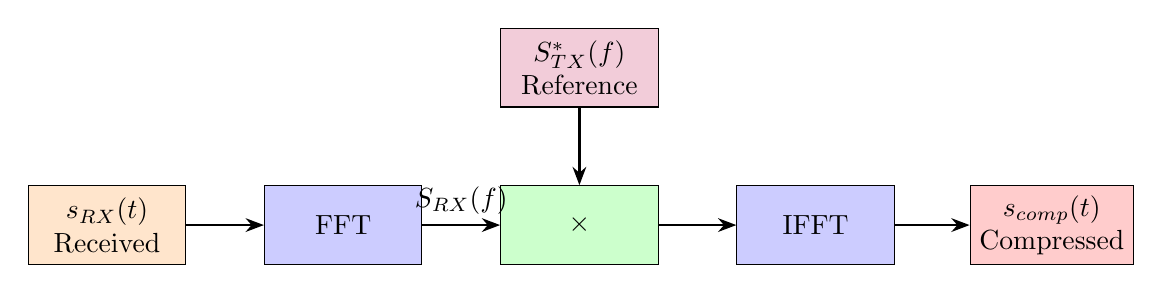
\begin{tikzpicture}[
    box/.style={rectangle, draw, minimum width=2cm, minimum height=1cm, align=center},
    arrow/.style={-{Stealth}, thick}
]
    % Input signal
    \node[box, fill=orange!20] (rx) at (0,0) {$s_{RX}(t)$\\Received};

    % FFT
    \node[box, fill=blue!20] (fft1) at (3,0) {FFT};

    % Multiply
    \node[box, fill=green!20] (mult) at (6,0) {$\times$};

    % Reference
    \node[box, fill=purple!20] (ref) at (6,2) {$S_{TX}^*(f)$\\Reference};

    % IFFT
    \node[box, fill=blue!20] (ifft) at (9,0) {IFFT};

    % Output
    \node[box, fill=red!20] (out) at (12,0) {$s_{comp}(t)$\\Compressed};

    % Arrows
    \draw[arrow] (rx) -- (fft1);
    \draw[arrow] (fft1) -- (mult) node[midway, above] {$S_{RX}(f)$};
    \draw[arrow] (ref) -- (mult);
    \draw[arrow] (mult) -- (ifft);
    \draw[arrow] (ifft) -- (out);

\end{tikzpicture}
\end{document}
